%%%%%%%%%%%%%%%%%%%%%%%%%
% Dokumentinformationen %
%%%%%%%%%%%%%%%%%%%%%%%%%


\newcommand{\trtitle}{App f\"ur Dienstabmachungen}
\newcommand{\scrartclScrreprt}{scrreprt}
%!TEX TS-program = pdflatex
\documentclass[fontsize=12pt]{\scrartclScrreprt}
\usepackage[utf8]{inputenc}

\usepackage[numbers]{natbib}
\usepackage{lmodern}
\usepackage[T1]{fontenc}
\usepackage[ngerman, num, orig]{isodate}
\usepackage[ngerman]{babel}   
\monthyearsepgerman{\,}{\,} 



% eigene commands

\newcommand{\texttodo}[1]{\textcolor{red}{Todo: #1}}


% Kompaktes Itemize
\usepackage{enumitem}
\newlist{compactitemize}{itemize}{1}
\setlist[compactitemize]{label=\textbullet, nosep, leftmargin=10pt}

\usepackage{layout}
\setlength{\parindent}{0em}

\usepackage{amssymb,amsmath,fancybox,graphicx,wrapfig,color,lastpage,fancyhdr,verbatim,epstopdf,a4wide}

\usepackage{tabularx}
\usepackage{setspace}
\usepackage{epsfig}
\usepackage{pst-pdf}
\usepackage{pst-all}
\usepackage{supertabular}{\tiny }
\usepackage[font=small,labelfont=bf]{caption}
\usepackage{subcaption}
\usepackage{footnote}
\usepackage{float}
\usepackage{multirow}
\usepackage{etex}
\usepackage{pdfpages}
\usepackage{color} 
\usepackage{placeins} 
\usepackage{booktabs}
\usepackage{pdflscape}

\usepackage[hyphens]{url}	%URL handling und darstellung
\urlstyle{tt}

\usepackage[pdftitle={\trtitle},
						pdfauthor={Philipp Riedel},
						pdfcreator={TexMate, LaTeX with hyperref},
						pdfsubject={\trtitle},
						plainpages=false,
						pdfpagelabels,
						colorlinks,
						linkcolor=black,
						filecolor=black,
						citecolor=black,
						urlcolor=blue]{hyperref}

\usepackage[makeroom]{cancel}
\usepackage{array}
\usepackage{trfsigns}
\usepackage{textcomp}

\title{\trtitle}
\subtitle{(Dokumentation)}
\author{(Philipp Riedel \& co)}

% Möglichst keine Ergänzungen hier, sondern in header.tex
\begin{document} 
 

% Römische Nummerierung für Sonderseiten, wie Verzeichnisse und Anhang
\pagenumbering{Roman}

% Titelblatt

\maketitle


% Inhaltsverzeichnis
\tableofcontents
\thispagestyle{empty}
% Nummerierung von roemisch auf arabisch umschalten und roemische
% zwischenspeichern
\newpage
\pagenumbering{arabic}

\section{Einleitung}

Diese Dokumentation soll während des ganzen Projekt ergänzt und nachgeführt werden.
\subsection{Zweck dieser Applikation}
\begin{itemize}
\item Diese App ist für Verkündiger gedacht.
\item Es soll nicht als Ersatz der Dienstabmachungen mit der eigenen Versammlung dienen.
\item Diese App soll lediglich das finden eines Dienstpartners vereinfachen, wenn Verkündiger eine kurzfristige Dienstabsage erhalten oder wenn niemand für den Dienst zu einer bestimmten Zeit gefunden werden konnte.
\item Die App hat ihr Anwendungsgebiet innerhalb einer bestimmten Region, welche im Moment auf den Raum Zürich beschränkt ist.
\item Diese App soll auch Abmachungen mit einer Sprache, die nicht der Muttersprache entspricht, ermöglichen.
\item Der Grundgedanke die Dienstgruppe und die Einheit zu fördern soll bei der Implementierung der Applikation berücksichtigt werden.
\end{itemize}

\subsection{Projektaufbau}

Dieser Aufbau ist noch abhängig von gewissen Grundsatzentscheiden, ausserdem ist er eventuell noch nicht Vollständig \texttodo{überarbeiten, nach vorgehens entscheid (cross plattform, je ein app, gwt usw.)}

\begin{center}
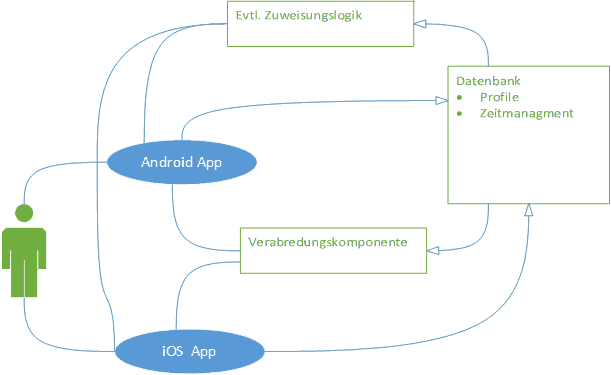
\includegraphics[width=0.75\textwidth]{bilder/useCase.png}
\end{center}

\section{Vorabklärungen}

\subsection{Zusammenfassung}
\begin{tabularx}{\textwidth}{lX}
Task  & Stand \\\hline
Bedürfnis & das Bedürfnis ist vorhanden \\
Teilnahme Abschätzung für Gelingen & Teilnehmerzahl $n \geqslant 100$, Pioniere $n_p \geqslant 50$\\
Aufwand & \texttodo{ToDo Cristian oder Anna-Nina} \\
Installation auf Android - und iOS Systeme & Android stellt kein Problem dar, bei AppStore fallen zusätzliche Kosten an, ausserdem ist man der Willkür von Apple ausgesetzt. Da aber viele ein iPhone besitzen muss auch für iOS eine App zur Verfügung gestellt werden.\\
Datenbank &\texttodo{Anna-Nina bitte eine Struktur vorschlagen, Aufwand, Unterhalt, Kosten und Risiken}\\
Sicherheit &  \texttodo{Philipp und Sam besprechung des Aufbaus der App mit einbezug von Theokratischen Argumenten}\\
\end{tabularx}

\subsection{Bedürfnis}

\paragraph{Wie gross ist das Bedürfnis nach dieser Applikation} bei vielen Verkündigern kommen Absagen relativ häufig vor, bei Pionieren 1 bis 2 mal pro Woche. Auch das finden von Abmachungen unter der Woche kann eine Herausforderung sein.

\subsection{Teilnahme Abschätzung für Gelingen}
\paragraph{Wie viele absagen braucht es pro Woche damit die Applikation einen Nutzen hat} Es gibt pro Tag in etwa die drei Hauptterminzeiten Morgen, Nachmittag und Abend. Samstag Abend wird weggelassen und sonntags zählt nur als eine Terminzeit. Somit ergeben sich 18 Termine pro Woche. Damit es öfters vorkommt das bei den Hauptterminzeiten eine Übereinstimmung mit $\pm\varepsilon$ gegeben ist, sollte mit 60 bis 100 Absagen oder nicht Finden einer Abmachung pro Woche gerechnet werden. Dies sollte mit einer Teilnehmerzahl $n \geqslant 100$ und davon $n_p \geqslant 50$ Pionieren erreicht werden.

\subsection{Aufwand}
\paragraph{Aufwand für Programmierung und Unterhalt} Der Aufwand muss im Verhältnis zum Nutzen stehen. \texttodo{Cristian oder Anna-Nina: bitte hier eine Zeitabschätzung getrennt nach Erstellen der Applikation sowie deren Unterhalt erstellen}

\subsection{Installation der App}
\paragraph{Bedignungen für die Installation auf Android - und iOS Systeme}
\begin{itemize}
\item Bei einem Android System ist es kein problem die Applikation auf ein File-Server zum Download anzubieten. Der Nutzer muss nur bei der Installation zustimmen, dass er die unbekannte App als vertrauenswürdig hält.
\item Bei einem iOS Stystem muss über den AppStore gegangen werden.  Zum Veröffentlichen der App im App Store ist eine kostenpflichtige Registrierung beim iOS Developer Program notwendig. Apple unterzieht jede eingesandte App einer Überprüfung und erteilt anschließend in der Regel die Freigabe für den App Store. Dies ist die einzige Möglichkeit die App zu verbreiten wenn die Apple Geräte keinem Jailbreak unterzogen wurden \cite{appStore}. Für das Anbieten von Apps im AppStore fallen kosten von 99.-\$ an.
\end{itemize}
Trotz Mehraufwand und zusätzlichen Kosten muss wegen der hohen Anzhal von iPhone besitzer auch für iOS eine App zur Verfügung gestellt werden.

\subsection{Datenbank}
\paragraph{Nutzen und Aufwand einer Datenbank}Da Profile erstellt werden müssen damit eine effiziente Zuordnung gemacht werden kann muss eine Datenbank Struktur vorhanden sein.

\texttodo{Anna-Nina bitte eine Struktur vorschlagen, Aufwand, Unterhalt, Kosten und Risiken}

\subsection{Sicherheit}
\paragraph{Abklärungen zur Sicherheit in Abhängikeit der Daten} Die Sicherheitsanforderungen hängen primär auch von den gespeicherten Daten ab. Die gespeicherten Attribute eines Verkündigers müssen noch Evaluiert werden, dies wird von Samuel Vontobel und Philipp Riedel mit eventueller Einbeziehung von weiteren Brüdern durchgeführt. Die Attribute sind wiederum abhängig von der Auslegung der Applikation. Telefonnummern werden zum Beispiel nicht benötigt wenn eine Appinterner Kommunikationsablauf zur Verabredung bereitgestellt wird. Namen würden z.B. nicht benötigt wenn eine Anonyme Zuweisung erfolgt. Eine Versammlungszugehörigkeit wird nur dann benötigt wenn bei einer automatischen Zuteilung die eigene Versammlung als Zulteilungspriorität gilt usw. 

\texttodo{Philipp und Sam besprechung des Aufbaus der App mit einbezug von Theokratischen Argumenten}\newline

\texttodo{Danach: Anna-Nina: Sicherheitsvorschlag, verschlüsselung? profile mit Password versehen? usw.}
\chapter{Entscheide}

\section{Entscheide zu Vorabklärungen}

\section{Entscheide zu technischen Fragen}

\section{Entscheide zu theokratischen Fragen}
\section{Software}

\subsection{Versionsverwaltung}
Es wird mit GIT gearbeitet (Turtorial\footnote{\url{https://www.kernel.org/pub/software/scm/git/docs/gittutorial.html}})und die Daten liegen auf git-hub{Repository\footnote{\url{https://github.com/priedel/dienstApp}}}. Das Projekt mit \enquote{git clone https://github.com/priedel/dienstApp.git} holen.
 Schreibrechte bei Philipp Riedel (E-Mail\footnote{\href{mailto:riedelp@student.ethz.ch}{riedelp@student.ethz.ch}}) beantragen.

\subsection{Programm Plattform}

Es gibt prinzipiell zwei Möglichkeiten. Pro Betriebssystem wird eine App entwickelt oder es wird mit einer Cross Plattform gearbeitet\cite{appEinf}.


\begin{tabularx}{\textwidth}{lX}
\textbf{individuell}\cite{appEinf}&\\
iOS & mit  Objective-C (oder C/C++)\\
Android & Java \\
\textbf{Cross Plattform}\cite{crossPlat}&\\
    RhoMobile & This is a solution that uses Ruby, especially loved by Ruby on Rails developers. (Free only for noncommercial applications, prices vary)\\
    Appcelerator & This is a solution that allows you to develop native apps with HTML/Javascript (run through a UIWebView on iPhone) . (Free)\\
    PhoneGap & Similar to Appcelerator, I mentioned these two as they seem to have the most vibrant communities, and most extensive support. (Free)\\
    WidgetPad & are good cross platform development tools. Out of these I would rather prefer Phonegap for iOS and Android Development.\\
	Xamarin \footnote{\url{http://www.phoronix.com/scan.php?page=news_item&px=MTUxMzA}}& Xamarin and Microsoft announced a global partnership that enables Microsoft developers to create native mobile Windows, iOS and Android apps with the language they know, C\#, and the tools they love, Visual Studio. This groundbreaking partnership empowers one of the world’s largest developer communities to become the most productive and innovative mobile developers – almost overnight.\\
	\multicolumn{2}{l}{\textbf{WEB mit Schnittstelle zu App oder Native}}\\
	GWT Project \footnote{\url{http://www.gwtproject.org/}} &
	GUI mit GWT zu machen und dann weitere Schnittstellen zu den Spezifischen App zu definieren. Oder GWT Native anzuwenden\\
\end{tabularx}
\centering{{$\vdots$}}

\subsection{Use Case diagramm}
\subsection{Klassendiagramm}

\subsection{Datenbank}



% Nummerierung wieder auf roemisch umschalten
%\newpage
%\pagenumbering{Roman}
%\setcounter{page}{\value{roemisch}}



\chapter{Verzeichnisse}
% Abbildungsverzeichnis
\addcontentsline{toc}{section}{Abbildungsverzeichnis}
\listoffigures

% Tabellenverzeichnis
\addcontentsline{toc}{section}{Tabellenverzeichnis}
\listoftables

% Literaturverzeichnis
\addcontentsline{toc}{section}{Literaturverzeichnis}
%\renewcommand{\refname}{Literaturverzeichnis}
\bibliographystyle{natdin}	%gerplain: [1], geralpha: [Bjar05]
\bibliography{./docFiles/Literatur}


% Appendix, falls vorhanden
\newpage
\numberwithin{table}{chapter}
\begin{appendix}
\section{....}
\end{appendix}


\end{document}
